% ----------------------------------------------------------------
% Article Class (This is a LaTeX2e document)  ********************
% ----------------------------------------------------------------
\documentclass[10pt]{article}
\usepackage[british]{babel}  %% Language
\usepackage[a4paper, margin=1in]{geometry} %% margins
\usepackage{graphicx} % Graphics - allows import of images
\usepackage{float} % Allows for control of float positions
\usepackage[a4paper,bookmarks=true, colorlinks=false]{hyperref} % Links - must be last package
\usepackage{algorithm}
\usepackage{natbib}
\usepackage[noend]{algpseudocode}

\providecommand{\keywords}[1]
{
  \small	
  \textbf{\textit{Keywords---}} #1
}
%----------------------------------------------------------------

% Title page

%----------------------------------------------------------------
\begin{document}
\title{\bf{Title}}%
%%%%
\author{Forename Surname \\ Student ID \\ Programme \\ National College of Ireland}%
%%% PLEASE UNDERLINE your surname as it appears in Moodle 


\date{}%
% ----------------------------------------------------------------
\maketitle
% ----------------------------------------------------------------


%----------------------------------------------------------------
% abstract
%----------------------------------------------------------------

\begin{abstract} 
The abstract goes here. You should provide a high-level \textbf{(up to 150 words)} overview of your proposed research work, its motivation, gaps in research you intend to fill, an indication of your research method and approach, and your expected contributions. This is the teaser of your work it'll probably be best to write it last.

\keywords{\textbf{Include 3-5 keywords} (separated by a comma) under the abstract that you feel capture the most important aspects of your paper}
 
\end{abstract}
%----------------------------------------------------------------
% Table of contents
%----------------------------------------------------------------
%\tableofcontents
%\thispagestyle{empty}
%\cleardoublepage
%\setcounter{page}{1}
%----------------------------------------------------------------
% Main Headings Section
%----------------------------------------------------------------

%%%%%%%%%%%%%%%%%%%%%%%%%%%%%%%%%%%%%%%%%%%%%%%%
\section{Introduction}  

In this section, you should provide introduce the topic of your research. You should describe the research problem that you are trying to solve (including its general context within your field of study), motivate why it is important to research the chosen topic, and outline what the general findings of the literature review are (such as the gaps in existing research). 
\\\\
Clearly identify the research question(s), and the proposed solution describing the potential contributions of your work and its benefits of your proposed solution (how it will contribute to knowledge in the field of research). 
\textbf{Research Question.} The above research problem motivates the following research question: How/What \textbf{[open-ended research question]}.
\\\\
Finally, include a paragraph describing the structure of your document (numbering the sections and outlining the key argument points you will be making in each section.)

%%%%%%%%%%%%%%%%%%%%%%%%%%%%%%%%%%%%%%%%%%%%%%%%
\section{Literature Review} 

The literature review is a critical analysis of the related work. It must compare, contrast, and relate previous work, enumerate the objectives of the previous work, and specify their foreseen contributions. 
In this section, you must introduce each previous work by outlining the key argument points that you will be covering, finish each subsection with a brief conclusion of what has been covered in the previous work, and then link to the next subsection by outlining what you will be discussing next.
\\\\
The literature review should be presented in a logical order of the reviewed previous works, critically contrast at least two previous works in each paragraph, as opposed to just “reciting” what the previous works say.  Every paragraph should explain what the significance of the previous works are in the context of your own research question. You must ensure there is consistent referral back to the research question (do not be afraid to consistently remind the reader why a point is relevant in the context of your own question). Finally, make sure the previous works are properly cited.
\\
Consider using various subheadings for presenting your literature review based on the classification or categorization you did of your papers.

\subsection{A meaningful subsection}
Add here your critical analysis for a group of papers

\subsection{Another meaningful subsection}
Add here your critical analysis for another group of papers

\subsection{Research Niche}
The literature review must finish identifying the research niche and the expected contribution of the research.

%%%%%%%%%%%%%%%%%%%%%%%%%%%%%%%%%%%%%%%%%%%%%%%%
\section{Research Methods \& Specifications} 

This section must describe your proposed methodological approach to the research as well as the expected/next research steps to bring your research project to completion. In this section, describe the proposed solution to your research question that will eventually underlie the implementation, and list and provide a brief explanation of the expected steps/activities planned to be carried out to bring your research project to completion during the Capstone project semester. 
\\\\
Include a Gantt chart for the project plan illustrating the tasks involved in the project and their order with the related dependencies against a timescale.
\\\\
Also, describe the tools and test data that you have identified as potentially useful in your research and validation. Finally, describe how you plan to evaluate your approach. You must describe how you plan to answer the research question that you pose and what evidence you will bring to support your claims/approach. That is, what experimental evidence you will bring to bear in order to show the effectiveness of your approach.
\\\\
Finally, identify and critically assess ethical issues surrounding the work you are proposing.
\\
An example of structure is below:

\subsection{Research Method}
This is an example of text

\subsection{Research Resources}
This is an example of text

\subsection{Evaluation}
This is an example of text

\subsection{Ethical Considerations of the Research}
This is an example of text

\subsection{Project Plan}

My plan to conduct my research plan is shown in Figure~\ref{fig:gantt}.

\begin{figure}[h]
\begin{center}
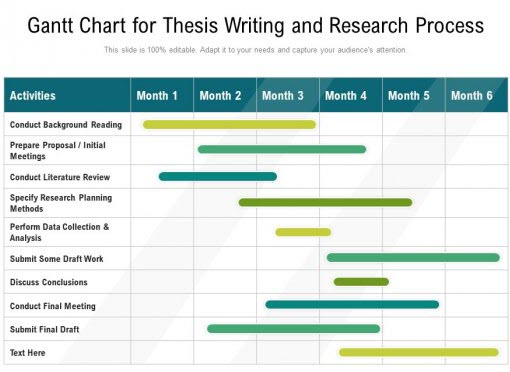
\includegraphics[width=0.8\textwidth]{CA2Img-GanttChart.jpg}
\caption{Project Plan for Research Work}
\label{fig:gantt}
\end{center}
\end{figure}

%----------------------------------------------------------------
% Bibliography section
%---------------------------------------------------------------
\newpage
%\bibliographystyle{ieeetr}
\bibliographystyle{agsm}
\bibliography{ricbib} 

\end{document}